 \documentclass[letterpaper,11pt]{article}
\oddsidemargin -1.0cm \textwidth 17.5cm

\usepackage[utf8]{inputenc}
\usepackage[activeacute,spanish]{babel}
\usepackage{amsfonts,setspace}
\usepackage{amsmath}
\usepackage{amssymb, amsmath, amsthm}
\usepackage{comment}
\usepackage{amssymb}
\usepackage{dsfont}
\usepackage{anysize}
\usepackage{multicol}
\usepackage{enumerate}
\usepackage{graphicx}
\usepackage[left=1.5cm,top=2cm,right=1.5cm, bottom=1.7cm]{geometry}
\setlength\headheight{1.5em} 
\usepackage{fancyhdr}
\usepackage{multicol}
\usepackage{hyperref}
\usepackage{wrapfig}
\pagestyle{fancy}
\fancyhf{}
\renewcommand{\labelenumi}{\normalsize\bfseries P\arabic{enumi}.}
\renewcommand{\labelenumii}{\normalsize\bfseries (\alph{enumii})}
\renewcommand{\labelenumiii}{\normalsize\bfseries \roman{enumiii})}

\begin{document}

\fancyhead[L]{\itshape{Facultad de Ciencias F\'isicas y Matem\'aticas}}
\fancyhead[R]{\itshape{Universidad de Chile}}

\begin{minipage}{11.5cm}
    \begin{flushleft}
        \hspace*{-0.6cm}\textbf{FI1000-5 Introducción a la Física Clásica}\\
        \hspace*{-0.6cm}\textbf{Profesora:} Paulina Lira\\
        \hspace*{-0.6cm}\textbf{Auxiliares:} Alejandro Silva, Felipe Kaschel, Juan Cristobal Castro\\
    \end{flushleft}
\end{minipage}

\begin{picture}(2,3)
    \put(405,-5){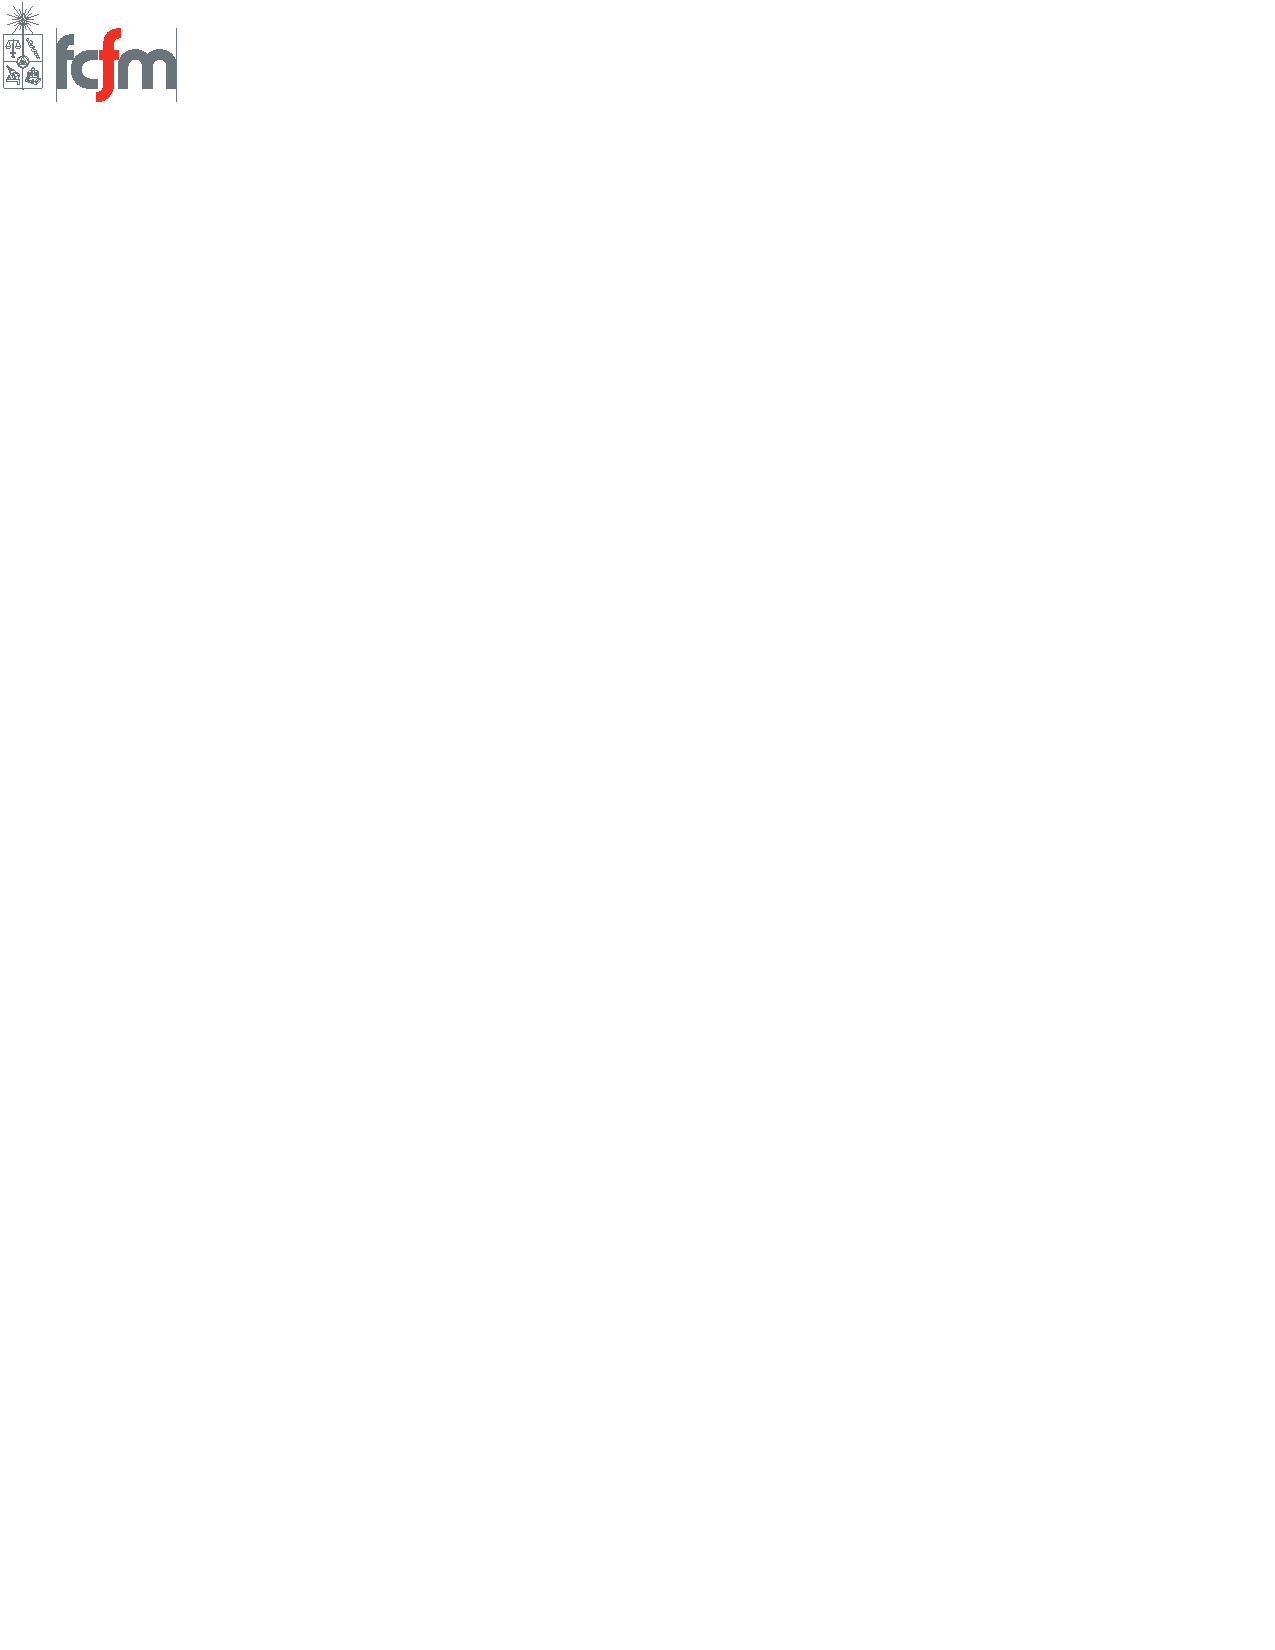
\includegraphics[scale=1.25]{2020-1/Imágenes/logo/fcfm2.pdf}}
\end{picture}

\begin{center}
	\LARGE \bf Auxiliar \#1: Trigonometría   \\
\end{center}

\vspace{-1cm}
\begin{enumerate}\setlength{\itemsep}{0.4cm}

\rfoot[]{pág. \thepage}

\item[]

\item Demuestre el teorema del seno y del coseno para un triángulo obtusángulo\\
\textit{Hint: forme un triángulo rectángulo}
\begin{figure}[h!]
    \centering
    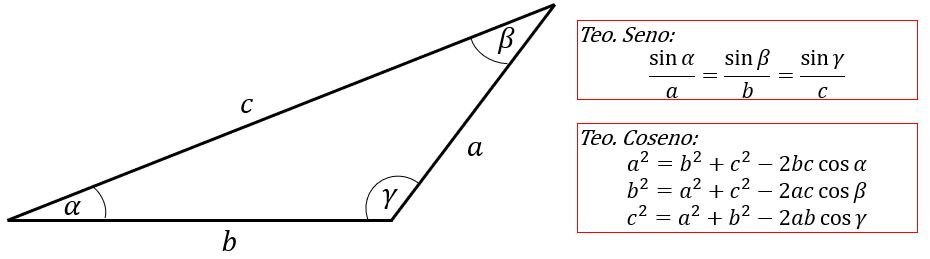
\includegraphics[scale = 0.4]{2020-1/Imágenes/aux1/teos.JPG}
\end{figure}

¿Cómo lo haría para un triángulo acutángulo?
    


\item Demuestre las siguientes relaciones trigonométricas: 
    \begin{enumerate}
        \item $\tan^2\alpha+1=\sec^2\alpha$
        
        \item $\cos^2\alpha=\cfrac{\cos(2\alpha)+1}{2}$
        
        \item $\cos \alpha+\cos\beta=2\cos\left(\cfrac{\alpha+\beta}{2}\right)\cos\left(\cfrac{\alpha-\beta}{2}\right)$
    \end{enumerate}
    
\item \href{https://www.geogebra.org/material/iframe/id/C6mhehH7/width/625/height/625/border/888888/sfsb/true/smb/false/stb/false/stbh/false/ai/false/asb/false/sri/false/rc/false/ld/false/sdz/false/ctl/false}{\textbf{Paralaje:}} Considere una estrella que se ubica perpendicularmente sobre el Sol. Encuentre una expresión para calcular la distancia Estrella-Sol utilizando el movimiento aparente de la estrella con respecto a las estrellas de fondo.
    \begin{figure}[h!]
        \centering
        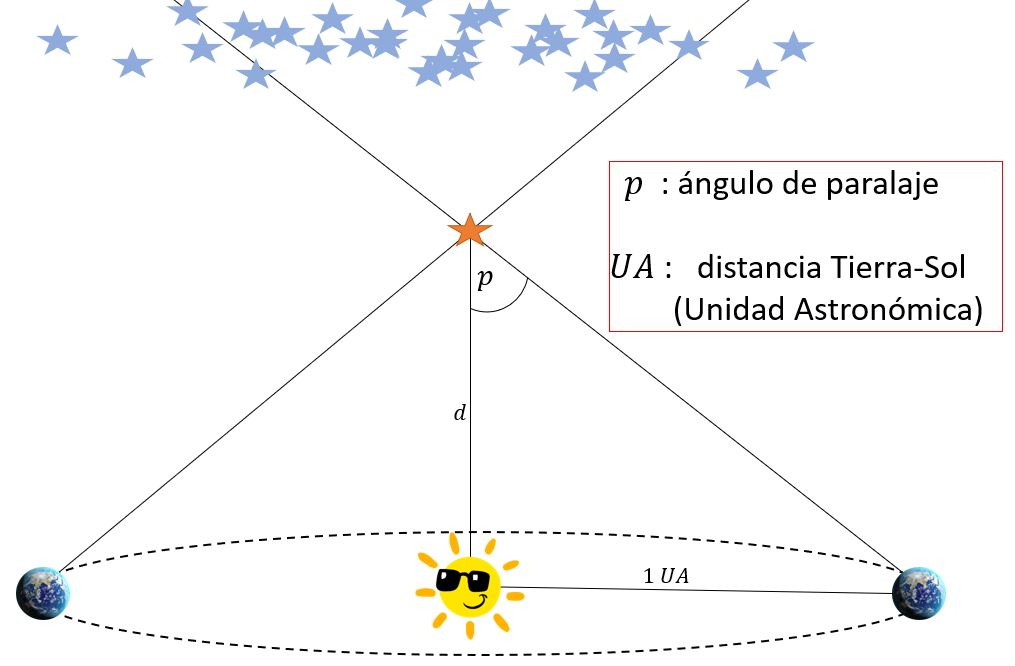
\includegraphics[scale=0.3]{2020-1/Imágenes/aux1/paralax.JPG}
    \end{figure}

\end{enumerate}
\end{document}